% abtex2-modelo-artigo.tex, v-1.9.2 laurocesar
% Copyright 2012-2014 by abnTeX2 group at http://abntex2.googlecode.com/ 
%

% ------------------------------------------------------------------------
% ------------------------------------------------------------------------
% abnTeX2: Modelo de Artigo Acadêmico em conformidade com
% ABNT NBR 6022:2003: Informação e documentação - Artigo em publicação 
% periódica científica impressa - Apresentação
% ------------------------------------------------------------------------
% ------------------------------------------------------------------------

\documentclass[
	% -- opções da classe memoir --
	article,			% indica que é um artigo acadêmico
	11pt,				% tamanho da fonte
	oneside,			% para impressão apenas no verso. Oposto a twoside
	a4paper,			% tamanho do papel. 
	% -- opções da classe abntex2 --
	%chapter=TITLE,		% títulos de capítulos convertidos em letras maiúsculas
	%section=TITLE,		% títulos de seções convertidos em letras maiúsculas
	%subsection=TITLE,	% títulos de subseções convertidos em letras maiúsculas
	%subsubsection=TITLE % títulos de subsubseções convertidos em letras maiúsculas
	% -- opções do pacote babel --
	english,			% idioma adicional para hifenização
	brazil,				% o último idioma é o principal do documento
	sumario=tradicional
	]{abntex2}

\usepackage[alf]{abntex2cite}
% PACOTES

\usepackage{lmodern}
\usepackage[T1]{fontenc}
\usepackage[utf8]{inputenc}
\usepackage{indentfirst}
\usepackage{nomencl}
\usepackage{color}	
\usepackage{graphicx}		
\usepackage{microtype}
\usepackage{siunitx}

\usepackage{lipsum}
		
\usepackage[brazilian,hyperpageref]{backref}
\bibliographystyle{plain}

% ---
% Configurações do pacote backref
% Usado sem a opção hyperpageref de backref
\renewcommand{\backrefpagesname}{Citado na(s) página(s):~}
% Texto padrão antes do número das páginas
\renewcommand{\backref}{}
% Define os textos da citação
\renewcommand*{\backrefalt}[4]{
	\ifcase #1 %
		Nenhuma citação no texto.%
	\or
		Citado na página #2.%
	\else
		Citado #1 vezes nas páginas #2.%
	\fi}%
% ---

% ---
% Informações de dados para CAPA e FOLHA DE ROSTO
% ---
\titulo{Bel e decibel, assim como suas variantes}
\autor{Henrique Marques de Carvalho Medeiros}
\local{Brasil}
\data{Maio de 2022}
% ---

% ---
% Configurações de aparência do PDF final

% alterando o aspecto da cor azul
\definecolor{blue}{RGB}{41,5,195}

% informações do PDF
\makeatletter
\hypersetup{
     	%pagebackref=true,
		pdftitle={\@title}, 
		pdfauthor={\@author},
    	pdfsubject={Modelo de artigo científico com abnTeX2},
	    pdfcreator={LaTeX with abnTeX2},
		pdfkeywords={abnt}{latex}{abntex}{abntex2}{atigo científico}, 
		colorlinks=true,       		% false: boxed links; true: colored links
    	linkcolor=blue,          	% color of internal links
    	citecolor=blue,        		% color of links to bibliography
    	filecolor=magenta,      		% color of file links
		urlcolor=blue,
		bookmarksdepth=4
}
\makeatother
% --- 

% ---
% compila o indice
% ---
\makeindex
% ---

% ---
% Altera as margens padrões
% ---
\setlrmarginsandblock{3cm}{3cm}{*}
\setulmarginsandblock{3cm}{3cm}{*}
\checkandfixthelayout
% ---

% --- 
% Espaçamentos entre linhas e parágrafos 
% --- 

% O tamanho do parágrafo é dado por:
\setlength{\parindent}{1.3cm}

% Controle do espaçamento entre um parágrafo e outro:
\setlength{\parskip}{0.2cm}  % tente também \onelineskip

% Espaçamento simples
\SingleSpacing

% ----
% Início do documento
% ----
\begin{document}

% Retira espaço extra obsoleto entre as frases.
\frenchspacing 

% ----------------------------------------------------------
% ELEMENTOS PRÉ-TEXTUAIS
% ----------------------------------------------------------

%---
%
% Se desejar escrever o artigo em duas colunas, descomente a linha abaixo
% e a linha com o texto ``FIM DE ARTIGO EM DUAS COLUNAS''.
% \twocolumn[    		% INICIO DE ARTIGO EM DUAS COLUNAS
%
%---
% página de titulo
\maketitle
% resumo em português
\begin{resumoumacoluna}
    Onda é um pulso que se propaga de um ponto a outro transportando energia sem transportar matéria. As ondas mecânicas são todas aquelas que dependem de um meio para se propagar e surgem em consequência da deformação de um meio elástico.
    O Bel Criado por conveniência, para expressar a razão de dois números com diferenças grandes.
    Os decibéis fazem o uso de logaritmos tornando estes números pequenos e fáceis de manipular, e transforma produtos em somas e divisões em subtrações.
 
 \vspace{\onelineskip}
 
 \noindent
 \textbf{Palavras-chaves}: Bel. Decibel. Onda Sonora. Medidas.
\end{resumoumacoluna}

% ]  				% FIM DE ARTIGO EM DUAS COLUNAS
% ---

% ----------------------------------------------------------
% ELEMENTOS TEXTUAIS
% ----------------------------------------------------------
\textual

% ----------------------------------------------------------
% Introdução
% ----------------------------------------------------------
\section*{Energia transportada pelas ondas}
\addcontentsline{toc}{section}{Introdução}

Todo e qualquer tipo de onda não transporta matéria. Onda é um pulso que se propaga de um ponto a outro transportando energia sem transportar matéria.

As ondas podem ser classificadas com relação à sua natureza de vibração como mecânicas e eletromagnéticas.

As ondas mecânicas são todas aquelas que dependem de um meio para se propagar e surgem em consequência da deformação de um meio elástico.
As ondas eletromagnéticas se propagam no vácuo e em alguns meios, surgem em consequência de cargas elétricas oscilantes\cite{demodelo}.

\section*{Intensidade do som}
\addcontentsline{toc}{section}{Intensidade do som}
A intensidade (I) de uma onda é basicamente a Potência transportada por uma unidade de área perpendicular ao
fluxo de energia.
$$I = \frac{Potência}{area} = \frac{(energia / tempo)} {area}$$

A intensidade I de um som pode ser percebida com precisão, e está relacionada com a quantidade de energia sonora recebida por segundo a partir da fonte de som. Os seres humanos podem perceber um amplo intervalo de intensidade, de $10^-12 Wm^-2$ até $100 Wm^{-2}$.

\begin{center}
    A energia é proporcional à amplitude ao quadrado:
\end{center}
$$I \propto A^2$$

Ao utilizar a energia para medir a intensidade do som, deve-se observar a potência sonora, onde potência [$1 Watt=1 J/s$] é trabalho em função do tempo. A Intensidade sonora é estabelecida pela potência aplicada em uma determinada área, no sistema SI $I=W.m^{-2}$ e no sistema CGS $I= erg.cm^{-2}.s^{-1}$

Quando utilizamos a pressão para medir a intensidade do som, a unidade de medida no SI é o Pascal [$1 Pa= 1 N*m-2$] e no sistema CGS a pressão é dada em $dyna*cm^-2$.

Um resultado importante de se trabalhar com nível de intensidade é que se a intensidade do som é dobrada, isso corresponde apenas a um aumento de 3 dB no nível de intensidade sonora. Mas, na prática é mais fácil medir variação de pressão do que intensidades.

\begin{table}[hb]
\centering
    \begin{tabular}{c  c  c}
Fontes de ruido & Intensidade ($Watt/m^2$) & dB\\ 
\hline
Limite da dor & $10^2$ & 140\\
\hline
Jato & $10^0$ & 120\\
\hline
Britadeira & $10^{-2}$ & 100\\
\hline
Via movimentada & $10^-4$ & 80\\
\hline
Escritório & $10^-6$ & 60\\
\hline
Residencial & $10^-8$ & 40\\
\hline
Estúdio de rádio operando & $10^-10$ & 20\\
\hline
Limite da audição & $10^-12$ & 0\\
\hline
    \end{tabular}
    \caption{Níveis sonoros}
\end{table}

O sistema auditivo do ser humano é muito sensível
e está preparado para receber sons de intensidades
muito baixas, da ordem de $10^-12 W/m2$ (ou seja,
0,000000000001 $W/m^2$) até intensidades tão altas
quanto 100 $W/m^2$.

\section{Bel}
\addcontentsline{toc}{section}{Bel}
Criado por conveniência, para expressar a razão de dois números com diferenças grandes. Homenagem ao cientista Alexander Graham Bell, inventor, entre outras, do telefone.

Onde é estabelecido que se a e b são dois níveis de potência, então a razão bel é: 
$$Nível de Potência = \log_{10} (a/b)$$

Logo, se a tem o dobro da potência de b então:
Nível de Potência= $\log_{10} 2 = .301 Bel$

\section{Decibel}
\addcontentsline{toc}{section}{DeciBel}

O dB é uma unidade logarítmica muito usada em telecomunicações, por pelo menos dois motivos : O ouvido humano tem resposta logarítmica (sensação auditiva versus potência acústica) e em telecomunicações, se usam números extremamente grandes ou pequenos. O uso de logaritmos torna estes números pequenos e fáceis de manipular, e transforma produtos em somas e divisões em subtrações.

O dB é um número relativo e permite representar relações entre duas grandezas de mesmo tipo, como relações de potências, tensões, correntes ou qualquer outra relação adimensional.
Portanto, permite definir ganhos e atenuações, relação sinal/ruído, dinâmica, etc...


\subsection{Nível de pressão sonora: decibel}
\addcontentsline{toc}{section}{Nível de pressão sonora:
decibel}

Para se medir o nível de pressão sonora é necessário uma pressão de referência, $P_0$. Usamos uma pressão sonora que é aproximadamente igual ao limiar de audibilidade a 1000 Hz, isto é, a pressão exercida por uma onda de som de um som de 1000 Hz no tímpano, que é apenas o suficiente para ser ouvida. Esta pressão é tomada como sendo $2 x 10^-5 N/m^2$. A escala de intensidade do som é então dada por:

$$SPL = 20 \log_{10}(P/P_0) dB$$

Nota-se que a fórmula para a escala usa $20 \log$ em vez de $10 \log$, já que a intensidade é proporcional ao quadrado da amplitude de pressão.

Utilizando-se a equação Fechner e Weber, e utilizando o nível de pressão sonora de referência como sendo $P_0 = \SI{20}{\micro}PA$ por ser esta a mínima pressão sonora audível por um indivíduo otologicamente normal e utilizando-se $K=20$, temos:

$$NPS = 20 \log (P/P_0)$$
$$\SI{20}{\micro}PA$$

\begin{table}[hb]
\centering
    \begin{tabular}{c c c}
$N/m^2$ & dB re $2 . 10^-5 N/m^2$)\\ 
\hline
200 & 140\\

20 & 120\\

2 & 100\\

$2 . 10^{-1}$ & 80\\

$2 . 10^{-2}$ & 60\\

$2 . 10^{-3}$ & 40\\

$2 . 10^{-4}$ & 20\\

$2 . 10^{-5}$ & 0\\

    \end{tabular}
    \caption{NPS ou SPL}
\end{table}

\subsection{Níveis de Intensidade e Pressão}
\addcontentsline{toc}{subsection}{Níveis de Intensidade e Pressão}
Os cálculos para o nível de pressão sonora, do inglês "Sound Pressure Level" são feitos em decibel.
$$SPL = 20 \log (P/P_{ref})$$
$$P_{ref} = 2.10^{-5} N/m^2$$
O Nível de Intensidade Sonora (Sound Intensity Level), também é calculado em decibel.
$$SIL = 10 \log (I/I_{ref})$$
$$I_{ref} = 10^{-12} Watt/m^2$$
Nível de Potência Sonora (Sound Power Level) assim como os outros é dado em decibel.
$$SWL = 10 \log (W/W_{ref})$$
Desse modo é possivel interligar as funções e dedusir logicamente que, se a intensidade sonora aumentar deum dado fator, a pressão média aumentará somente a raiz quadrada desse fator. Além de que se a pressão sonora aumentar de um dado fator, a intensidade sonora aumentará o quadrado daquele fator.
$$P \propto \sqrt{I}$$
$$I \propto P^2$$
$$I = \frac{P^2}{Z_c}$$

\section{Qualidade sonora}
Sylvio Bistafa fez uma estudo para descobrir a qualidade de autos falantes com base em experimentos empíricos e definiu que:
\begin{citacao}
Um alto-falante suspenso no ar gera som, porém de baixa qualidade acústica. Isso significa qualidade do som falante não atende às expectativas do ouvinte.\cite{bistafa2018acustica}
\end{citacao}
Isso se relaciona diretamente com o conceito humano para a qualidade sonora que se baseia em cinco pilares principais. São eles a altura,a intensidade ou sonoridade, o timbre a sensação sonora.

\addcontentsline{toc}{section}{Qualidade de um som}
\subsection{Altura}
É a qualidade do som que nos permite distinguir os sons graves dos agudos.
\subsection{Intensidade ou Sonoridade do Som}
É a qualidade que nos permite distinguir os sons fortes dos fracos. Volume perceptível do som.
\subsection{Timbre}
É a qualidade que nos faz distinguir as vozes de duas pessoas, mesmo quando emitindo sons de mesma frequência.
Também permite diferenciar os sons de dois instrumentos musicais, mesmo quando eles emitem a mesma nota.

\subsection{Sensação sonora}
A sensação sonora varia aproximadamente com o logaritmo da pressão sonora.
O nosso ouvido não reage igualmente para todas as frequências sonoras.
A sensibilidade varia, e muito, com a frequência do som.
Dois sons de mesma intensidade física mas frequências diferentes podem parecer, para o nosso ouvido, ter intensidades muito diferentes.

\begin{figure}[h]
\caption{Curvas de igual audibilidade ou
isofônicas}
\centering % para centralizarmos a figura
\includegraphics{Curvas de igual audibilidade.jpg} % leia abaixo
\label{Curvas de igual audibilidade ou
isofônicas}
\end{figure}

\subsection{Sensibilidade do Ouvido}
\begin{figure}[h]
\caption{Curvas de igual audibilidade ou
isofônicas}
\centering % para centralizarmos a figura
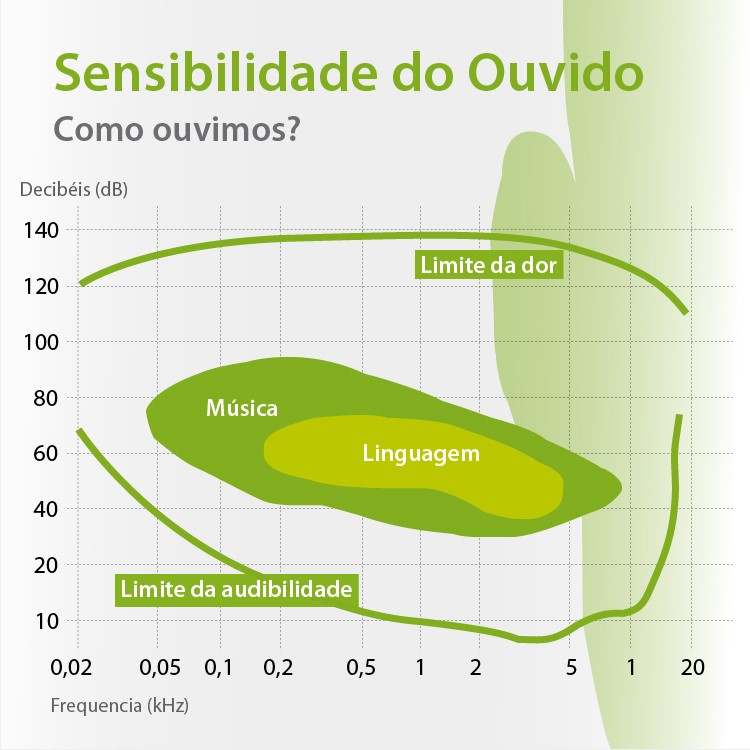
\includegraphics[width=200]{Limiar de audição.jpg} % leia abaixo
\label{Curvas de igual audibilidade ou
isofônicas}
\end{figure}

\begin{figure}[h]
\caption{Curvas de igual audibilidade ou
isofônicas}
\centering % para centralizarmos a figura
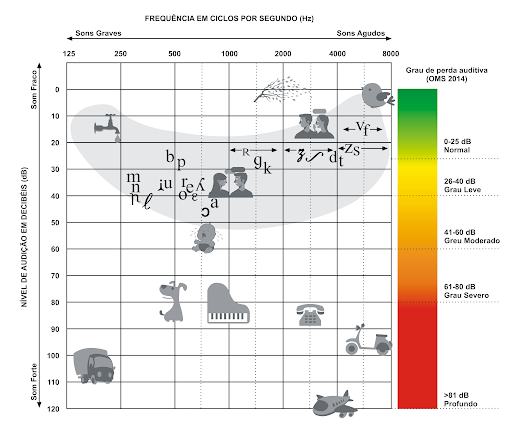
\includegraphics{Audiograma de sons.png} % leia abaixo
\label{Curvas de igual audibilidade ou
isofônicas}
\end{figure}

O aparelho auditivo, concentrado no interior da cabeça, é dividido em três partes. A primeira parte é o ouvido externo, onde se encontra o canal auditivo. A segunda parte é ouvido médio, também conhecido como cavidade timpânica, onde se localiza o tímpano e os ossículos. A terceira parte é o ouvido interno, onde se concentra a cóclea o nervo auditivo.

Para que consigamos fazer a recepção do som, é preciso que a onda sonora entre pelos ouvidos externos e percorra um canal auditivo até chegar ao tímpano. Com a presença dessas ondas sonoras, o tímpano começa a vibrar. Nesse momento, os dois ossos da cavidade timpânica, o martelo e a bigorna acionam outro osso chamado de estribo, que transfere essa informação ao ouvido interno.

Ao passar por cada um desses obstáculos, as ondas sonoras são aplicadas e vão em direção ao caracol do ouvido. Nesse local existem células nervosas do nervo auditivo que enviam os sinais das ondas sonoras ao cérebro. É nesse instante que temos a percepção do som.

\section{Outras unidades logarítmicas}
\subsection{dBA}
Zero dBA equivale a uma intensidade sonora (pressão sonora) de
20 microPascal, e equivale aproximadamente ao limiar de audição. O limiar de
dor se situa em torno de 120 dBA, ou seja, uma pressão 1 000 000 de vezes
maior ou uma potência sonora 1 000 000 000 000 de vezes maior ! (a potência
sonora é proporcional ao quadrado da pressão). O A se refere a um tipo de
filtro de ponderação (weighting), que leva em conta a não linearidade do ouvido
em freqüência. A figura seguinte mostra a curva de ponderação "A". 
Aintensidade sonora também pode ser medida sem essa ponderação, em dB ou
dBZ, em relação à referencia de 20 microPascal = 0 dB. Por exemplo, um som
com freqüência de 100 Hz e intensidade de 60 dBA tem uma intensidade não
ponderada de 79 dB, pois a curva A apresenta 19 dB de atenuação em 100 Hz.
Em 1000 Hz (e 6000 Hz), as medidas em dB e dBA são idênticas.

\subsection{Neper}
Uma unidade bastante usada em calculo é o Neper, que é igual ao logaritmo neperiano da razão de duas tensões (ou correntes) na mesma impedância. Obs: $1 N = 8,65 dB.$

\begin{citacao}
O neper, Np, é utilizado para expressar os valores de grandezas cujos valores numéricos se baseiam no uso do logaritmo neperiano (ou natural), ln = loge . O bel, B, e o decibel, dB, onde 1 dB = (1/10) B, são utilizados para expressar os valores de
grandezas logarítmicas cujos valores numéricos se baseiam no uso do logaritmo na
base 10, onde lg = log10 . A maneira como essas unidades são interpretadas está
descrita nas notas (g) e (h) da tabela 8. Raramente é necessário se atribuir um valor
numérico para essas unidades. As unidades neper, bel e decibel foram aceitas
pelo CIPM para uso com o SI, mas não são consideradas como unidades SI.\cite{santos2012sistema}
\end{citacao}

\subsection{dBr}
É uma unidade relativa de medida de nível, em relação ao ponto zero de transmissão, (0 TLP), onde geralmente o nível do tom de teste é de 0 dBm.
Apenas indica o somatório dos ganhos e atenuações num ponto qualquer em relação ao ponto de referencia, ou ponto zero de transmissão.

\subsection{dBm}
É uma unidade de medida de potência : $0 dBm = 1 mW$ (Não importa em qual resistência !)
$$P (dBm) = 10 log P (mW)$$
Portanto : 
$$3 dBm = 2 mW$$ $$30 dBm = 1W$$ $$-30 dBm = 1 \mu W$$

\subsection{dBm0}
É uma unidade de medida de potência relativa ao ponto zero.
Geralmente, é usado para indicar o nível de outros sinais, como pilotos, tons de sinalização, ruído, fuga de portadora, diafonia, etc., em relação ao tom de teste.

\subsection{dBp}
dB ponderado psofometricamente (psofos= ruído), ou seja, que leva
em conta o somatório das respostas em frequência do ouvido e da cápsula
receptora telefônica, e usado para medir ruído e relações sinal/ruído em
telefonia. Aplica-se também ao $dBm > dBmp e dBm0 > dBm0p$

\subsection{dBi}
Usado para expressar o ganho de uma antena em relação a antena ISOTRÓPICA. A antena isotrópica tem um diagrama de irradiação esférico, ou seja, irradia igualmente em todas as direções. O dBi é muito usado em cálculos de enlaces de telecomunicações, pois a atenuação de propagação é sempre calculada entre antenas isotrópicas. A antena isotrópica é uma referencia teórica, sendo de difícil construção prática.

\subsection{dBd}
Usado para expressar o ganho de uma antena em relação ao DIPOLO de meia onda. O dipolo de meia onda é a antena ressonante mais simples e fácil de ser construída e por isso é muito usada como referencia. Em espaço livre, o ganho do dipolo de meia onda é de $0 dBd = 2,15 dBi$

% Conclusão

\section*{Considerações finais}
\addcontentsline{toc}{section}{Considerações finais}

Conclui-se que essas unidades de medida foram criadas para uma melhor conspeção das vibrações sonoras, e são utilizadas comumente em todos os campos da ciência para a aferição de tais proporções.


% ELEMENTOS PÓS-TEXTUAIS
\postextual

% Título e resumo em língua estrangeira

% INICIO DE ARTIGO EM DUAS COLUNAS

% titulo em inglês
\titulo{Bel and decibel, as well as their variants}
\emptythanks
\maketitle

\renewcommand{\resumoname}{Abstract}
\begin{resumoumacoluna}
 \begin{otherlanguage*}{english}
   A wave is a pulse that travels from one point to another transporting energy without transporting matter. Mechanical waves are all those that depend on a medium. To propagate and arise as a result of the deformation of an elastic medium. Bel Created for convenience, to express the ratio of two numbers with large differences. Decibels make use of logarithms making these numbers small and easy to manipulate, and turns products into additions and divisions into subtractions.

   \vspace{\onelineskip}
 
   \noindent
   \textbf{Key-words}: Bel. Decibel. Sound wave. Measurements.
 \end{otherlanguage*}  
\end{resumoumacoluna}

%FIM DE ARTIGO EM DUAS COLUNAS

% Referências bibliográficas

\bibliography{abntex2-modelo-references}

\end{document}